%%%%%%%%%%%%%%%%%%%%% DO NOT MODIFY THIS PART
\documentclass[a4paper, 10pt]{article}
\usepackage[T1]{fontenc}
\usepackage{helvet} 
\renewcommand{\rmdefault}{phv}  % 设置 Helvetica 为默认字体
\renewcommand{\seriesdefault}{m}  % 确保字体系列为 m(正常粗细)
\usepackage{lmodern}
\usepackage{mathptmx}
\usepackage[x11names]{xcolor}
\usepackage[colorlinks, urlcolor=DodgerBlue3, linkcolor=DarkOrchid3, citecolor=DarkOrchid3]{hyperref}
\usepackage{indentfirst}
\usepackage[english]{babel}
\usepackage[utf8]{inputenc}
\usepackage{csquotes}
\usepackage[bitstream-charter]{mathdesign}
\usepackage{bm}
\usepackage{amsmath}
%zhichizhongwen
\usepackage{xeCJK}  % 支持中文
% 设置中文和西文的字体
\setCJKmainfont{Microsoft YaHei}
\setmainfont{Times New Roman}
\usepackage{booktabs}
\usepackage{graphicx}
\usepackage{siunitx}
\usepackage{float}
\usepackage{physics}
\usepackage{multirow}
%%%%%%%%画三线表实用的包
\usepackage[utf8]{inputenc}
\usepackage{multicol}
\usepackage{multirow}
\usepackage{booktabs}
\usepackage{threeparttable}
\usepackage{array}
%%%自动格式化设置
\usepackage{setspace}
\onehalfspacing  % 1.5 倍行距
\doublespacing   % 2 倍行距
%%自动调整表格、公式、段落等对齐
\usepackage{amsmath}
\usepackage{array}
\usepackage[backend=biber, maxbibnames=5, minbibnames=3, style=numeric-comp, sorting=none, url=false, isbn=false, doi=false]{biblatex}
\usepackage{xpatch}
\renewbibmacro{in:}{}
\DeclareFieldFormat{pages}{#1}
\newbibmacro{string+doiurl}[1]{%
	\iffieldundef{doi}{
		\iffieldundef{url}{#1}
		{\href{\thefield{url}}{#1}}
	}{\href{http://dx.doi.org/\thefield{doi}}{#1}}}
\DeclareFieldFormat[article]{title}{\usebibmacro{string+doiurl}{#1}}
\AtEveryBibitem{%
	\clearlist{language}%
	\clearfield{month}
	\clearfield{number}
	\clearfield{note}}
\newbibmacro{date+pages}{%
	\printfield{pages}%
	\setunit*{\space}%
	\usebibmacro{date}%
	\setunit*{\addcomma\space}%
	\newunit}
\xpatchbibdriver{article}
{\newunit
	\usebibmacro{note+pages}}
{}{}{}
\renewbibmacro*{journal+issuetitle}{%
	\usebibmacro{journal}%
	\setunit*{\addspace}%
	\iffieldundef{series}
	{}
	{\newunit
		\printfield{series}%
		\setunit{\addspace}}%
	\usebibmacro{volume+number+eid}%
	\newunit
	\usebibmacro{note+pages}%
	\setunit{\addspace}%
	\usebibmacro{issue+date}%
	\setunit{\addcolon\space}%
	\usebibmacro{issue}%
	\newunit}


\usepackage{titling}
\pretitle{\begin{center} \huge \bfseries}
	\posttitle{\par \end{center} \vspace{-\baselineskip} }
\preauthor{\begin{center} \large}
	\postauthor{\par *\href{mailto:\corremail}{\corremail} \end{center} \vspace*{-1.5cm}}
\usepackage{authblk}
\renewcommand\Affilfont{\itshape}
\pagenumbering{gobble}
\date{}
%%%%%%%%%%%%%%%%% DO NOT MODIFY ANYTHING ABOVE THIS LINE
%%%%%%%%%%%%%%%%%%%%%%%%%%%%%%%%%%%%%%%%%%%%%%%%%%%%%%%%


% Enter here your title and the authors with their affiliations. For subscripts or superscripts use \textsubscript{} and \textsuperscript{} as in the example below.
\title{
	Summary of Research Achievements %% Put your title here
}

\author[1,*]{XXX}
\affil[1]{Computer Science and Technology, Zhejiang University, Hangzhou, China}
\def \corremail{12421094@zju.edu.cn} % give your email here

%% \author[1]{Second Author}
%%\author[2]{Third Author}
%\affil[2]{Department name, Another institution, Another city, Country}

\begin{document}
\maketitle % DO NOT REMOVE THIS LINE
\begin{abstract}
	这篇文章主要用来梳理我的研究成果和思路想法,这句话为了证明本文档可以支持中文!% 中文内容
	Your abstract text goes here. The abstract should be between 150 to 300 words and should provide a concise overview of the problem, methodology, main results, and conclusions.
\end{abstract}


\section{to-do}


\subsection{database}
Exploring QUIC Dynamics: A Large-Scale Dataset for  Encrypted Traffic Analysis,待论文录取后数据集公开



\subsection{A novel QUIC traffic classifier based on convolutional neural networks}

1.based on the convolutional neural network which combines the feature extraction and classification phase into one system.
\begin{figure}[ht]
	\centering
	\begin{minipage}{0.5\textwidth}% 小页面尺寸,可自行调节
		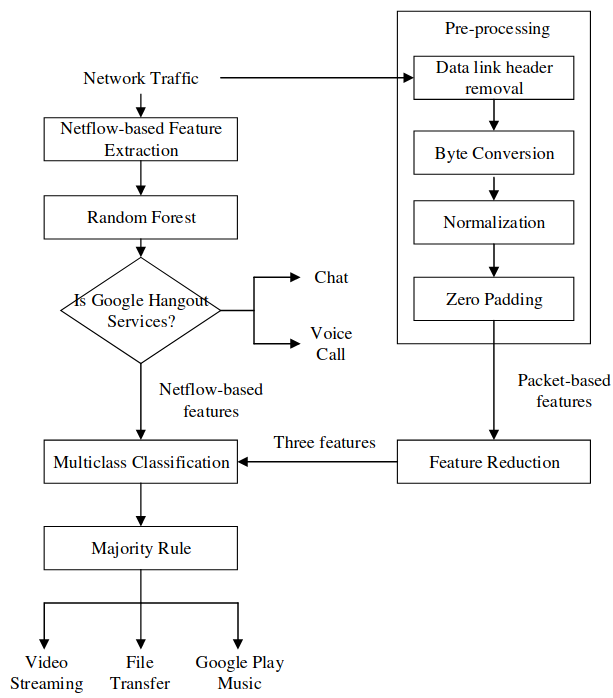
\includegraphics[width=6cm]{1205.jpg}
		\caption{The structure of this database}
		\label{fig:cnn}
	\end{minipage}
\end{figure}






\section{to read}

Lee, J., et al. (2023). "Challenges and Solutions in Identifying QUIC Traffic." Proceedings of the ACM Conference on Network Traffic Analysis.

Zhang, Y., \& Chen, L. (2023). "Using Machine Learning to Detect QUIC Traffic." International Journal of Network Security.

Singh, A., et al. (2024). "Flow-level Identification of QUIC Traffic using Heuristic Methods." Computer Networks Journal.

Patel, R., \& Roy, D. (2023). "Hybrid DPI and Flow Analysis for QUIC Traffic." IEEE Transactions on Network and Service Management.

Kim, S., et al. (2023). "The Privacy Trade-offs in QUIC Traffic Identification." Journal of Privacy and Security Research.

He, Y., et al. (2024). "Adapting Traffic Analysis for Evolving QUIC Versions." Journal of Protocol Engineering.

\section*{main points and key words}




\section{Video Datasets}

1、An Encrypted Network Video Stream.
Available online 22 June 2023 	~
\href{file://D:/database/envsds/envsds.zip}{the local storage path} ~
\href{https://zenodo.org/records/8039729/files/envsds.zip?download=1}{The url that I downloaded the database}
author:捷克理工大学信息技术学院\\
the structure is showed in the figure \ref{fig:database1}.

\begin{figure}[ht]
	\centering
	\begin{minipage}{0.5\textwidth}% 小页面尺寸,可自行调节
		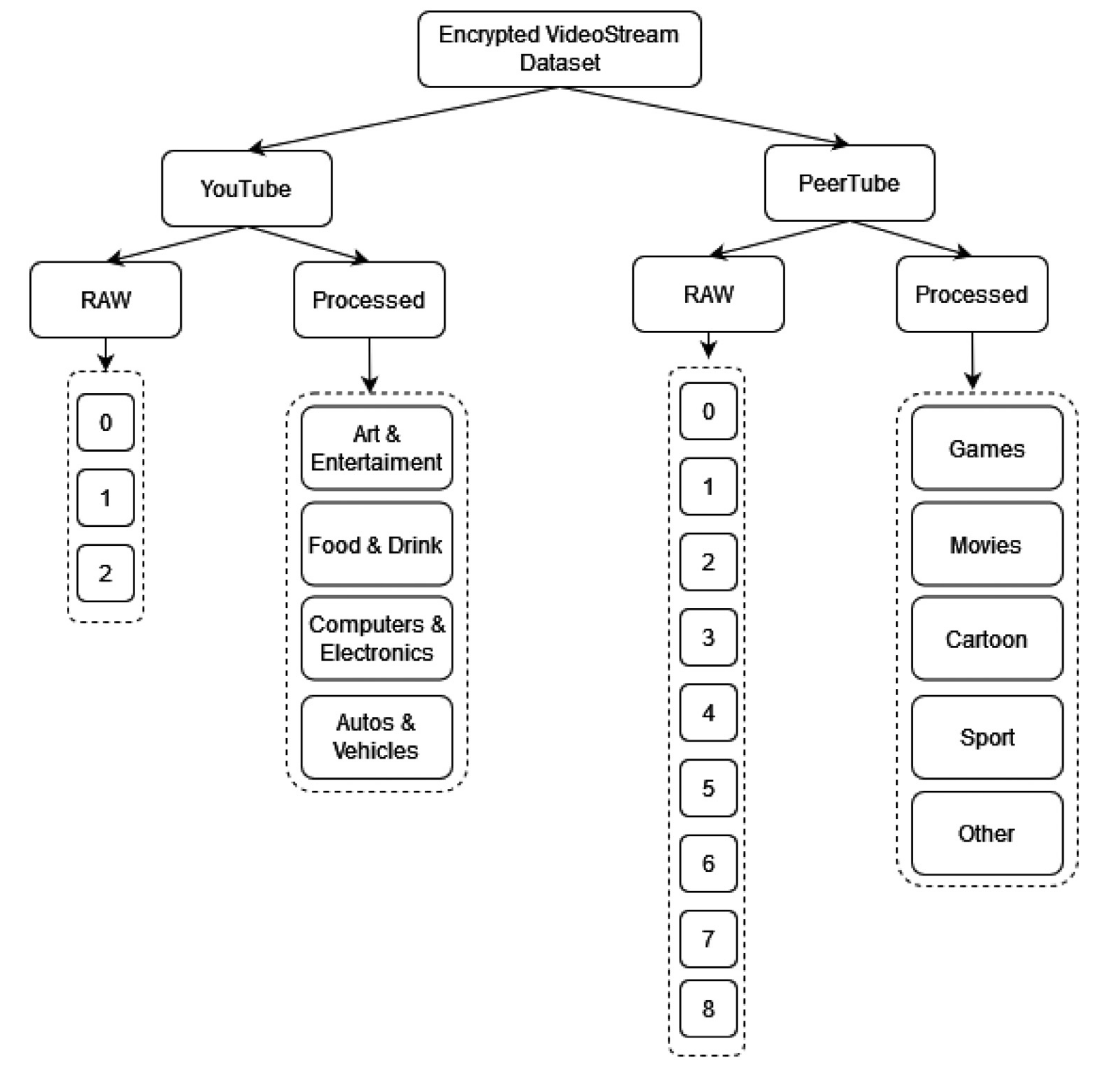
\includegraphics[width=6cm]{database1.jpg}
		\caption{The structure of this database}
		\label{fig:database1}
	\end{minipage}
\end{figure}


\section{QUIC}
\subsection{QUIC protocol}

One of QUIC’s main features is a fast connection establishment: In the ideal case,  when cached information of a prior connection is available, it does not even take a single  round-trip (0-RTT) to send encrypted application data. Yet, in the worst case (without  prior connections as in our measurements), QUIC needs at least three round-trips as  shown in Figure \ref{fig:quic1} and explained next.


\begin{figure}[ht]
	\centering
	\begin{minipage}{0.8\textwidth}% 小页面尺寸,可自行调节
		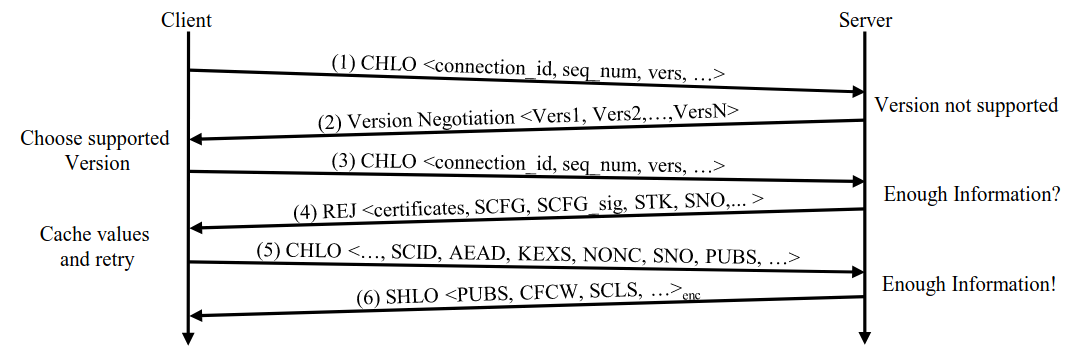
\includegraphics[width=500pt]{quic1.png}
		\caption{The structure of this database}
		\label{fig:quic1}
	\end{minipage}
\end{figure}

Clients initiate a connection using a Client Hello (CHLO)(1) including the QUIC  version it desires to use. In case the server does not support this version, it may send  a version negotiation packet (2) enabling the client to choose from a list of supported  versions for a second try. We will utilize packet (1) to quickly probe for QUIC-capable  hosts with only a single packet exchange and analyze their supported versions provided  in (2). Using a supported version, the client may advance in the handshake by sending  another CHLO (3), without prior communication, it does not possess enough information  about the server to establish a valid connection. The server supplies the necessary  information (4), in one or multiple exchanges (i.e., (3) and (4) may be repeated until all  required data is available). In these step(s), the client will be given a signed server config  (SCFG) including supported ciphers, key exchange algorithms and their public values,  and among other things the certificates authenticating the host. We will utilize these  information to analyze the server-provided certificates. With this information, the client  can issue another CHLO (5) including enough information to establish a connection, the  client may even send encrypted data following the CHLO which depicts the optimal case  for a 0-RTT connection establishment. Following the CHLO, the server acknowledges (6)  the successful connection establishment with a Server Hello (SHLO), containing further  key/value-pairs enabling to fully utilize the connection. from [A First Look at QUIC in the Wild]


\subsection{特点}

加密性:QUIC 使用了 TLS 1.3 进行端到端加密,这意味着所有的数据包都经过加密处理,流量特征在网络中难以直接进行内容分析。

基于 UDP:QUIC 基于 UDP 协议进行传输,绕过了传统的 TCP 流量分析方法。

流量混淆:QUIC 流量在传输过程中具有较高的混淆性,尤其是通过 TLS 1.3 加密的传输数据,使得基于传统的端口号、协议类型等特征进行分类变得更加困难。

\subsection{挑战}

流量特征不明显:由于 QUIC 使用了加密和混淆技术,传统基于数据包内容(如协议字段、端口号等)的方法无法有效地识别 QUIC 流量。
TLS 加密头的变化:虽然 QUIC 使用了 TLS 1.3 协议进行加密,但其协议头结构与传统的 HTTPS 协议相比有所不同,导致加密流量识别变得更加复杂。
UDP 的多路径特性:QUIC 支持多路径传输(multipath),这意味着同一会话的数据包可以通过不同的路径发送,进一步增加了流量分析的复杂度。








\section{Deep Packet Inspection (DPI) Challenges}

As QUIC encrypts much of its traffic, it presents a challenge for traditional traffic analysis methods such as DPI. Researchers have explored several techniques to analyze QUIC traffic, such as looking at timing patterns and side-channel information, bypassing encryption restrictions.(Source: Lee et al., 2023), explores the challenges of using traditional DPI with QUIC and presents methods to decode QUIC traffic without needing full decryption, by analyzing the connection establishment phase.
\section{Machine Learning for Traffic Classification}

Machine learning has been increasingly applied to classify QUIC traffic. By training classifiers on features like packet sizes, timing, and flow duration, researchers have developed systems that can identify QUIC flows without needing to decrypt them.
(Source: Zhang \& Chen, 2023) discusses applying machine learning for traffic identification and its potential to overcome the encryption challenges imposed by QUIC, even in the presence of packet fragmentation.


\section{Flow-Level Identification Techniques}

Several techniques aim at distinguishing QUIC flows from traditional TCP/UDP flows based on unique characteristics like flow-level behavior or handshakes. One significant development is analyzing the QUIC handshake phase, which is distinct and can often be used for identification.
(Source: Singh et al., 2024), in their work on flow identification, introduces new heuristics that focus on QUIC's handshake pattern, which could be leveraged by network operators to detect QUIC traffic early.
\section{Enhanced DPI Approaches with QUIC-specific Features}

Despite QUIC's encryption, there are still several identifiable features within the packet headers that can be exploited for traffic classification. Researchers are developing DPI tools that combine these features with machine learning to detect QUIC traffic more effectively.
(Source: Patel \& Roy, 2023), introduces a hybrid approach combining DPI and flow analysis, which can identify QUIC traffic by leveraging non-encrypted portions of the QUIC handshake.
\section{Privacy and Anonymity Concerns}
As QUIC's design emphasizes privacy and low latency, there is ongoing research into whether traffic classification efforts compromise these principles. Researchers argue that excessive reliance on identification techniques might undermine the core advantages of QUIC.
(Source: Kim et al., 2023) discusses the trade-off between privacy, security, and traffic identification in QUIC networks, suggesting potential solutions for maintaining anonymity without compromising network analysis.
\section{Protocol Analysis and Evolution}
There have also been studies focusing on the evolving nature of QUIC itself. As new versions of QUIC are introduced (like QUICv2), there are concerns about the adaptability of existing traffic identification techniques.
(Source: He et al., 2024) investigates the evolution of QUIC and provides a comprehensive overview of how traffic analysis must adapt to the upcoming versions of the protocol.

\section{Hybrid Approaches for Identification}
Hybrid methods combining DPI, machine learning, and statistical analysis are being developed to identify QUIC traffic. These methods aim to strike a balance between accuracy and minimal interference with encryption mechanisms.
(Source: Gupta \& Zhao, 2023), presents a hybrid methodology that uses both DPI and timing analysis to improve identification accuracy for QUIC traffic, even when encrypted.

\section{measurement}
The F1-score-
\[
	\begin{array}{c|c|c}
		\text{}     & \text{实际正例(Positive)} & \text{实际负例(Negative)} \\
		\hline
		\text{预测正例} & TP                    & FP                    \\
		\text{预测负例} & FN                    & TN                    \\
	\end{array}
\]



\[
	F1 = 2 \cdot \frac{\text{Precision} \cdot \text{Recall}}{\text{Precision} + \text{Recall}}
\]
其中:
\[
	\text{Precision} = \frac{\text{TP}}{\text{TP} + \text{FP}}
\]
\[
	\text{Recall} = \frac{\text{TP}}{\text{TP} + \text{FN}}
\]

\begin{figure}[ht]
	\centering
	\begin{minipage}{0.8\textwidth}% 小页面尺寸,可自行调节
		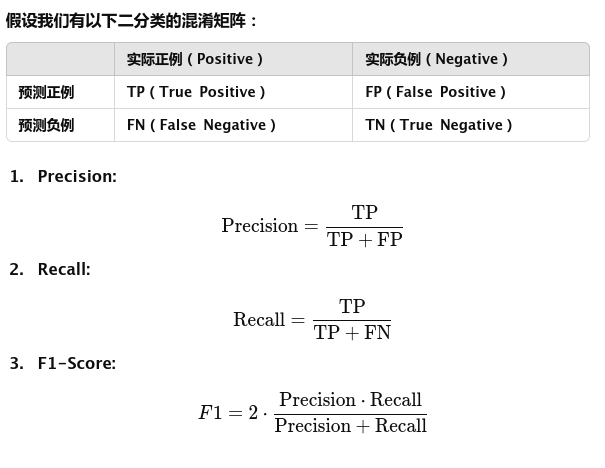
\includegraphics[width=15cm]{F1.jpg}
		\caption{The structure of this database}
		\label{fig:F1score}
	\end{minipage}
\end{figure}






\section{old cotent,just for template}
Start by giving some motivations, then describe your work and your results. Accents can be written directly without any trouble as for instance the village of Vogüé in Ardèche. For units, siunitx is loaded, so do not hesitate to write about your high magnetic field of \SI{9}{\tesla} or your spin waves with frequencies up to \SI{250}{\GHz}, or even your spatial resolution in the \si{\nano\meter} range. You can add equations like this, and refer to them (see Eq.~\ref{eq:topo_charge}):
\begin{equation}
	\label{eq:topo_charge}
	Q_\text{topo} = \frac{1}{4\pi} \int \vec{m}(\vec{r}) \cdot \left (\pdv{\vec{m}}{x} \times \pdv{\vec{m}}{y} \right) \dd{\vec{r}}
\end{equation}

For references, that you may cite like this\cite{wolfSpintronicsSpinBasedElectronics2001}, use the Bibtex format in a file named \texttt{biblio.bib} and use biber as a compiler. You can get the Bibtex description from Zotero or from a DOI on this website: \url{https://www.doi2bib.org/}.  The references section will then be filled automatically. We also suggest to add a nice figure with some caption to catch the attention of your audience (see Fig.~\ref{fig:spin}), following this example:
\begin{figure}[ht]
	\centering
	
\includegraphics[width=6cm]{111.jpg}
	\caption{This is a spin, or maybe a chestnut.}
	\label{fig:spin}
\end{figure}

Note that you can use figures in any usual format (tif, png, jpg... and even pdf), you simply need to upload the corresponding file in your Overleaf project. The size of the figure can easily be chosen with the ``width'' parameter.

Once you are ready, go to \href{https://cln2025.sciencesconf.org/}{the conference website} to upload your pdf abstract as the main file. This pdf file can be downloaded from Overleaf by clicking on the ``Download PDF'' icon in the right pannel (next to the ``Recompile'' button). \textbf{As a supplementary file, we ask you to upload a .zip file containing your .tex file, together with your biblio.bib file and your figure(s) (if any)}. Such a zip can be downloaded directly from Overleaf: in the (top left) overleaf Menu, click to download the Source; or from the project list that you see on your Overleaf home page (when clicking on the Home icon), you can click on the download icon which indicates ``Download .zip file''. \textbf{\textcolor{Firebrick1}{This is mandatory, we need these files to create the final booklet.}}




\begin{table*}[!htp] \footnotesize
	\centering
	\fontsize{6.5}{8}\selectfont
	\begin{threeparttable}
		\caption{xxxxxx.}
		\label{1234567}
		\setlength{\tabcolsep}{15mm}
		\begin{tabular}{ccccccc}
			\toprule
			\multirow{2}{*}{me} &
			\multicolumn{3}{c}{nihao}\cr
			\cmidrule(lr){2-4}
			                    & xx         & xx         & xxe\cr
			\midrule
			%%%%%%%%% kinect%%%%%%%  ZED
			xx                  & 73$\%$     & 66$\%$     & 68$\%$\cr
			%4D&0.7321&0.7222&0.7311&0.6243&0.6227&0.6570\cr
			xxxx                & 9$\%$      & 73$\%$     & 91$\%$\cr
			xxxx                & 9$\%$      & 75$\%$     & 1$\%$\cr
			xxx                 & 91$\%$     & 89.78$\%$  & 92.28$\%$\cr
			xxx                 & {\bf9$\%$} & {\bf7$\%$} & {\bf9$\%$}\cr
			\bottomrule
		\end{tabular}
	\end{threeparttable}
\end{table*}
















\section*{Acknowledgments}
If you wish to acknowledge people or funding, do it there.

%%%%%%%%%%%%% REFERENCES
\printbibliography
% Text of the abstract
Text of the abstract (one page maximum, including references).

% The bibliography. BibTeX can also be used.
\begin{thebibliography}{60}
	\bibitem{just a template}template,
	\textit{teest}
	\bibitem{codd} Codd, E. F. (1983). A relational model of data for large shared data banks. \textit{Communications of the ACM}, 26(1), 64--69.

\end{thebibliography}



\end{document}